\documentclass[aspectratio=169,10pt]{beamer}

\usepackage[T1]{fontenc}
\usepackage[utf8]{inputenc}
\usepackage[french]{babel}
\usepackage{lmodern}
\usepackage{graphicx}
\usepackage{booktabs}
\usepackage{array}
\usepackage{tabularx}
\usepackage{tikz}
\usepackage{xcolor}

\graphicspath{
  {../rapport/images/}
  {../rapport/diagrams/}
  {../preview/}
}

\definecolor{heigred}{HTML}{D0002B}
\definecolor{deepblue}{HTML}{17324D}
\definecolor{softblue}{HTML}{E8F1F8}
\definecolor{softred}{HTML}{FBE9ED}
\definecolor{softgreen}{HTML}{E8F5EE}
\definecolor{textgray}{HTML}{333333}
\definecolor{mutedgray}{HTML}{6B7280}
\definecolor{linegray}{HTML}{D7DEE8}

\usetheme{default}
\usefonttheme{professionalfonts}
\setbeamertemplate{navigation symbols}{}
\setbeamertemplate{itemize item}{\raisebox{0.15ex}{\scriptsize\textcolor{heigred}{$\blacktriangleright$}}}
\setbeamertemplate{itemize subitem}{\scriptsize\textcolor{deepblue}{$\bullet$}}
\setbeamertemplate{frametitle}{
  \vspace{0.25cm}
  \begin{beamercolorbox}[wd=\paperwidth,leftskip=0.55cm,rightskip=0.55cm]{frametitle}
    \usebeamerfont{frametitle}\insertframetitle
    \ifx\insertframesubtitle\empty\else
      \\[-0.1cm]{\usebeamerfont{framesubtitle}\textcolor{mutedgray}{\insertframesubtitle}}
    \fi
  \end{beamercolorbox}
  \vspace{-0.05cm}
  \hspace{0.55cm}\textcolor{linegray}{\rule{0.91\paperwidth}{0.4pt}}
}
\setbeamertemplate{footline}{
  \leavevmode
  \hbox{
    \begin{beamercolorbox}[wd=.73\paperwidth,ht=2.4ex,dp=1.1ex,leftskip=0.55cm]{author in head/foot}
      \scriptsize\textcolor{mutedgray}{Scanner 3D -- rapport intermédiaire}
    \end{beamercolorbox}
    \begin{beamercolorbox}[wd=.27\paperwidth,ht=2.4ex,dp=1.1ex,rightskip=0.55cm plus1fil]{date in head/foot}
      \scriptsize\textcolor{mutedgray}{\insertframenumber/\inserttotalframenumber}
    \end{beamercolorbox}
  }
}

\setbeamercolor{normal text}{fg=textgray,bg=white}
\setbeamercolor{frametitle}{fg=deepblue,bg=white}
\setbeamerfont{frametitle}{series=\bfseries,size=\Large}
\setbeamerfont{framesubtitle}{size=\small}
\setbeamerfont{title}{series=\bfseries,size=\huge}
\setbeamerfont{subtitle}{size=\large}

\newcommand{\tagbox}[2]{%
  \tikz[baseline=(n.base)]\node[
    rounded corners=2pt,
    fill=#1,
    inner xsep=5pt,
    inner ysep=2pt
  ] (n) {\scriptsize\bfseries #2};%
}

\newcommand{\validbox}[1]{%
  \begin{beamercolorbox}[wd=\linewidth,sep=0.25cm,rounded=true]{}
    \colorbox{softgreen}{%
      \parbox{\dimexpr\linewidth-0.5cm\relax}{\textbf{\textcolor{deepblue}{Validé}}\quad #1}%
    }
  \end{beamercolorbox}
}

\newcommand{\limitbox}[1]{%
  \begin{beamercolorbox}[wd=\linewidth,sep=0.25cm,rounded=true]{}
    \colorbox{softred}{%
      \parbox{\dimexpr\linewidth-0.5cm\relax}{\textbf{\textcolor{heigred}{Limite}}\quad #1}%
    }
  \end{beamercolorbox}
}

\newcommand{\nextbox}[1]{%
  \begin{beamercolorbox}[wd=\linewidth,sep=0.25cm,rounded=true]{}
    \colorbox{softblue}{%
      \parbox{\dimexpr\linewidth-0.5cm\relax}{\textbf{\textcolor{deepblue}{Suite}}\quad #1}%
    }
  \end{beamercolorbox}
}

\newcommand{\placeholder}[2]{%
  \begin{center}
  \begin{tikzpicture}
    \node[
      draw=linegray,
      dashed,
      rounded corners=3pt,
      fill=softblue,
      minimum width=0.96\linewidth,
      minimum height=#1,
      align=center,
      text width=0.86\linewidth,
      inner sep=8pt
    ] {
      \textbf{\textcolor{deepblue}{Image à ajouter}}\\[0.15cm]
      \small #2
    };
  \end{tikzpicture}
  \end{center}
}

\newcommand{\maturity}[2]{%
  \begin{tikzpicture}[baseline=-0.6ex]
    \foreach \x in {1,...,5} {
      \ifnum\x>#1
        \filldraw[fill=white,draw=linegray] (\x*0.18,0) circle (0.055);
      \else
        \filldraw[fill=#2,draw=#2] (\x*0.18,0) circle (0.055);
      \fi
    }
  \end{tikzpicture}
}

\title{Scanner 3D à triangulation laser}
\subtitle{Présentation intermédiaire -- Projet multidisciplinaire}
\author{Luc Marchand \and Tim Stamm \and Jason Weber \and Hadrien Fuentes \and Tom Berthoud}
\institute{HEIG-VD -- PMD 2026}
\date{28 avril 2026}

\begin{document}

{
\setbeamertemplate{footline}{}
\begin{frame}
  \begin{columns}[T,onlytextwidth]
    \begin{column}{0.48\textwidth}
      
\includegraphics[height=1.35cm]{HEIG-VD_logo.png}
    \end{column}
    \begin{column}{0.48\textwidth}
      \raggedleft
\includegraphics[height=1.35cm]{logo_hesso.pdf}
    \end{column}
  \end{columns}

  \vspace{1.0cm}
  {\usebeamerfont{title}\textcolor{deepblue}{Scanner 3D à triangulation laser}}\\[0.25cm]
  {\usebeamerfont{subtitle}\textcolor{mutedgray}{Rapport intermédiaire -- démonstration de prototype}}\\[0.55cm]

  \begin{tikzpicture}
    \fill[heigred] (0,0) rectangle (1.1,0.08);
    \fill[deepblue] (1.18,0) rectangle (5.8,0.08);
  \end{tikzpicture}

  \vfill
  \small
  \textbf{Équipe :} Luc Marchand, Tim Stamm, Jason Weber, Hadrien Fuentes, Tom Berthoud\\
  \textbf{Contexte :} Projet multidisciplinaire HEIG-VD, semestre 4\\
  \textbf{Date :} 28 avril 2026
\end{frame}
}

\begin{frame}{Pourquoi ce projet ?}{Un outil ouvert pour le MakeLab}
  \begin{columns}[T,onlytextwidth]
    \begin{column}{0.54\textwidth}
      \begin{itemize}
        \item Numériser des objets physiques en modèles 3D exploitables.
        \item Obtenir un fichier \textbf{STL ou OBJ} sans chaîne logicielle propriétaire.
        \item Proposer un système compréhensible, modifiable et maintenable par des étudiants.
        \item Garder un budget compatible avec un projet PMD.
      \end{itemize}

      \vspace{0.35cm}
      \validbox{La valeur du projet n'est pas seulement le résultat 3D : c'est aussi une chaîne de mesure explicable de bout en bout.}
    \end{column}
    \begin{column}{0.42\textwidth}
      \placeholder{4.8cm}{Photo souhaitée : contexte MakeLab ou prototype posé sur une table, avec l'objet à scanner visible. Nom conseillé : \texttt{proto\_contexte.jpg}.}
    \end{column}
  \end{columns}
\end{frame}

\begin{frame}{Cahier des charges}{Les contraintes qui pilotent la conception}
  \begin{columns}[T,onlytextwidth]
    \begin{column}{0.49\textwidth}
      \begin{tabularx}{\linewidth}{@{}>{\bfseries}p{2.7cm}X@{}}
        \toprule
        Objet & Jusqu'à $150\times150\times150$ mm \\
        Temps & Scan complet en moins de 10 min \\
        Export & STL ou OBJ obligatoire \\
        Usage & Prise en main en moins de 10 min \\
        Interface & Web et/ou USB, retour visuel \\
        Budget & Environ 300 CHF \\
        \bottomrule
      \end{tabularx}
    \end{column}
    \begin{column}{0.46\textwidth}
      \begin{itemize}
        \item La boîte fermée limite la lumière ambiante et protège l'utilisateur.
        \item Les LEDs et l'écran indiquent l'état du scanner.
        \item La sécurité laser reste une contrainte non négociable pour la version utilisateur.
      \end{itemize}

      \vspace{0.3cm}
      \tagbox{softred}{Point critique}\quad Interlock capot encore à intégrer.
    \end{column}
  \end{columns}
\end{frame}

\begin{frame}{Principe de triangulation laser}{Un profil 3D par position angulaire}
  \begin{columns}[T,onlytextwidth]
    \begin{column}{0.46\textwidth}
      \begin{enumerate}
        \item Le plateau tourne pas à pas.
        \item Le laser ligne éclaire un profil de l'objet.
        \item La caméra capture la déformation de la ligne.
        \item Le pixel détecté est projeté en point 3D.
        \item Les profils sont fusionnés sur $360^\circ$.
      \end{enumerate}

      \vspace{0.2cm}
      \nextbox{La qualité finale dépend directement de ce que la caméra voit réellement.}
    \end{column}
    \begin{column}{0.50\textwidth}
      \begin{tikzpicture}[scale=0.92, every node/.style={font=\small}]
        \draw[fill=softblue,draw=linegray] (0,0) rectangle (6.25,4.45);

        % Vue image : la ligne laser reste verticale, mais son abscisse
        % varie avec la profondeur du profil de la pièce.
        \draw[fill=white,draw=linegray,thick] (0.45,0.55) rectangle (2.35,3.95);
        \node[deepblue] at (1.4,4.18) {image caméra};
        \draw[mutedgray,densely dotted] (1.4,0.75) -- (1.4,3.75);
        \draw[heigred,very thick]
          (1.25,0.8)
          .. controls (1.72,1.25) and (1.05,1.7) .. (1.55,2.15)
          .. controls (1.95,2.55) and (1.28,3.0) .. (1.72,3.65);
        \node[align=center,text width=1.8cm] at (1.4,0.2) {\scriptsize ligne verticale\\[-0.04cm]\scriptsize décalée par le profil};

        % Vue pseudo-3D : le plan laser est vertical et droit.
        \coordinate (cam) at (5.65,3.55);
        \draw[fill=white,draw=mutedgray] (3.0,0.65) -- (5.25,1.0) -- (5.95,0.65) -- (3.7,0.3) -- cycle;
        \draw[->,mutedgray,thick] (4.55,0.62) arc (205:-35:0.58 and 0.18);
        \node[mutedgray] at (4.55,0.1) {\scriptsize plateau};

        \draw[fill=softred,draw=heigred,very thick,opacity=0.42]
          (3.25,0.55) -- (4.05,0.80) -- (4.05,3.78) -- (3.25,3.48) -- cycle;
        \draw[heigred,very thick] (3.25,0.55) -- (3.25,3.48);
        \draw[heigred,very thick] (4.05,0.80) -- (4.05,3.78);
        \node[heigred,align=center] at (3.65,4.05) {plan laser\\vertical};

        \draw[fill=white,draw=deepblue,thick]
          (4.55,0.95) .. controls (5.05,1.28) and (4.25,1.6) .. (4.8,1.98)
          .. controls (5.35,2.36) and (4.45,2.72) .. (4.98,3.12)
          -- (5.28,1.0) -- cycle;
        \node[deepblue] at (5.12,0.72) {\scriptsize pièce};

        \coordinate (q1) at (3.76,1.03);
        \coordinate (q2) at (3.86,1.62);
        \coordinate (q3) at (3.73,2.18);
        \coordinate (q4) at (3.91,2.88);
        \draw[fill=white,draw=deepblue,thick] (cam) circle (0.15);
        \draw[deepblue,thick] (5.48,3.38) -- (5.10,3.08) -- (5.46,2.95) -- cycle;
        \node[deepblue,anchor=west] at (5.78,3.55) {caméra};
        \foreach \q in {q1,q2,q3,q4} {
          \draw[deepblue!65,thin] (cam) -- (\q);
          \fill[heigred] (\q) circle (0.045);
        }
        \draw[heigred,very thick]
          (q1) .. controls (3.96,1.25) and (3.68,1.42) .. (q2)
               .. controls (3.58,1.88) and (3.98,2.32) .. (q3)
               .. controls (4.05,2.55) and (3.72,2.72) .. (q4);
        \node[align=center,text width=2.25cm] at (5.03,2.35) {\scriptsize profil éclairé\\[-0.04cm]\scriptsize dans le plan};
      \end{tikzpicture}
    \end{column}
  \end{columns}
\end{frame}

\begin{frame}{Architecture globale}{Une chaîne modulaire de la capture à l'export}
  \begin{columns}[T,onlytextwidth]
    \begin{column}{0.70\textwidth}
      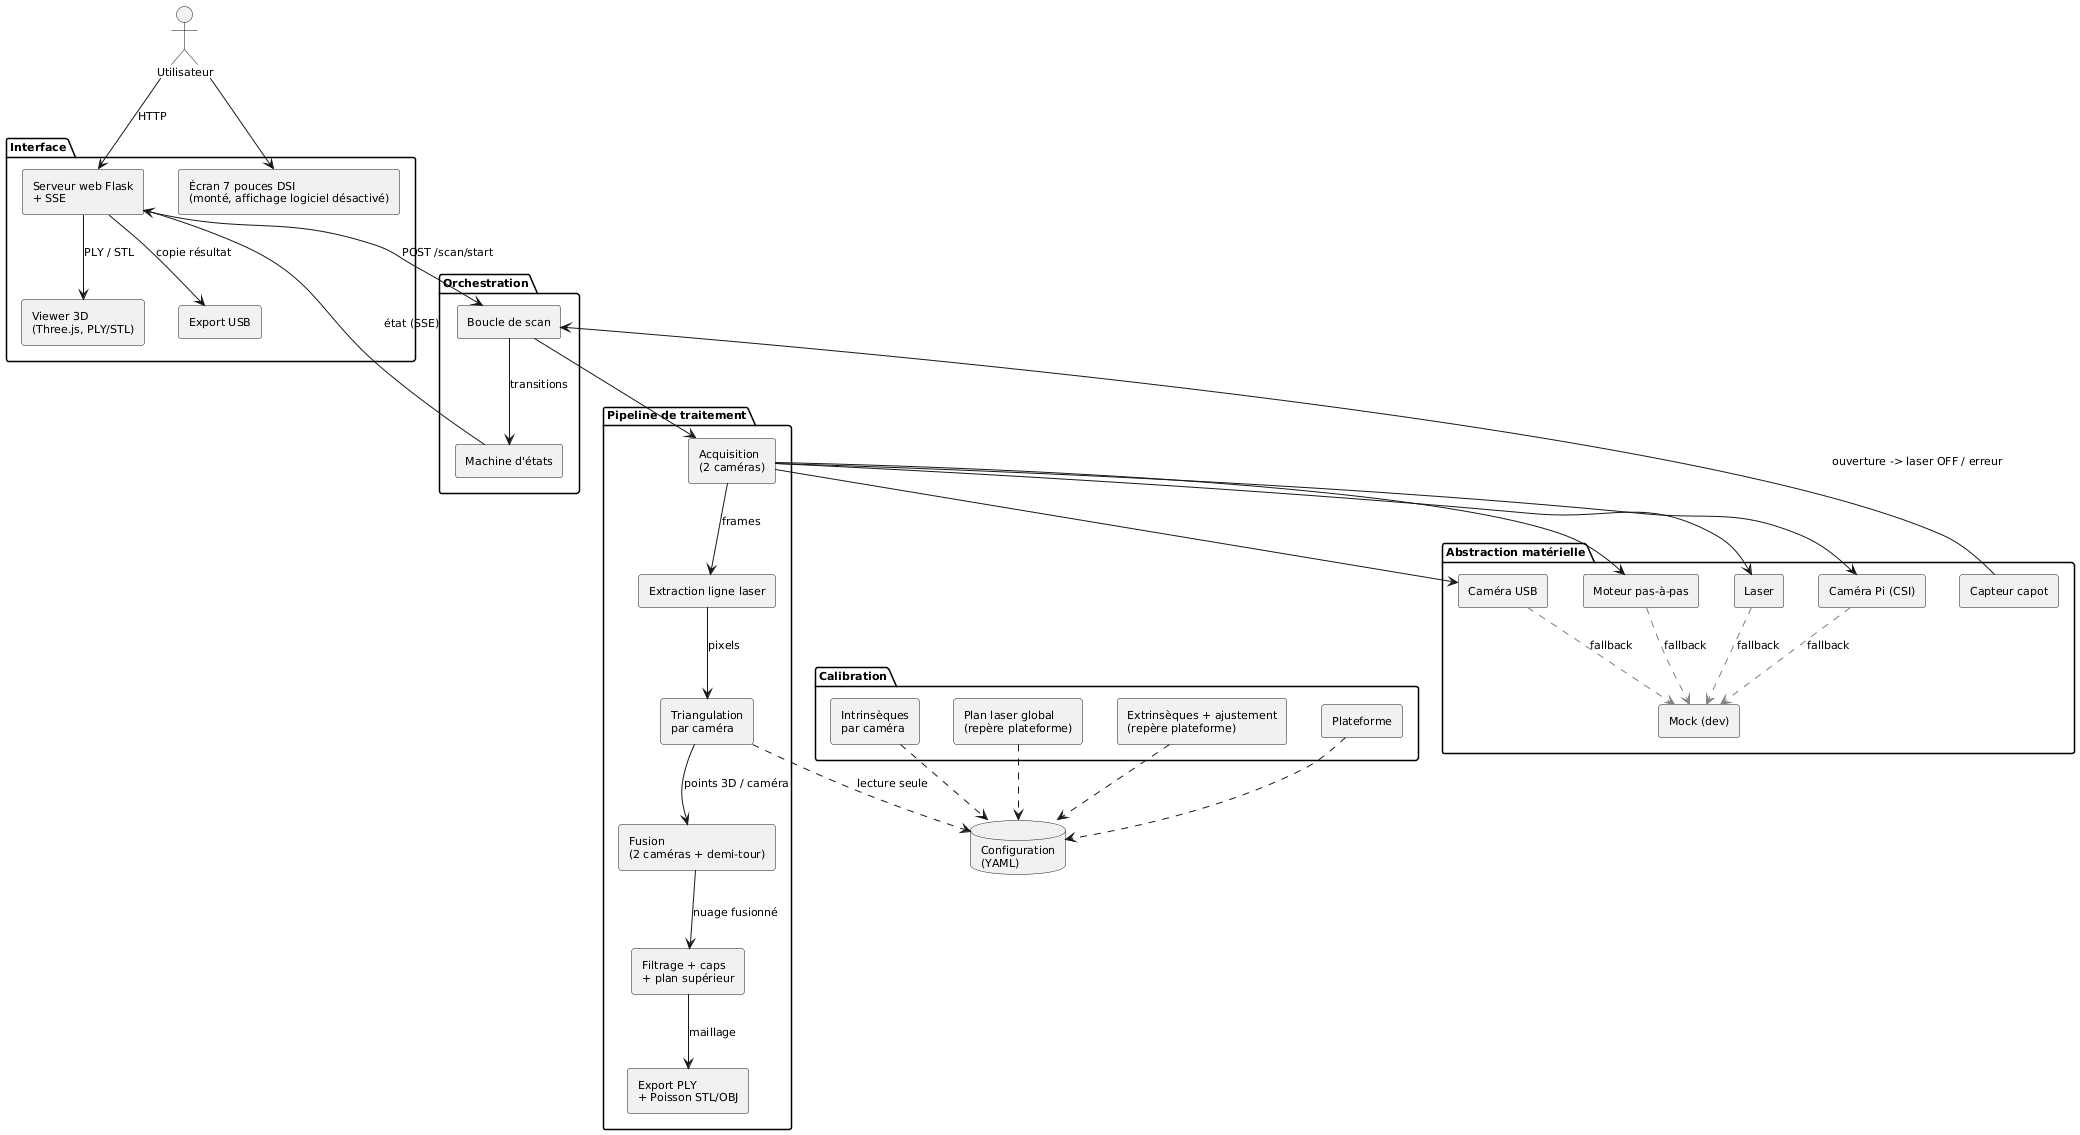
\includegraphics[width=\linewidth,height=6.0cm,keepaspectratio]{architecture_composants.png}
    \end{column}
    \begin{column}{0.26\textwidth}
      \small
      \begin{itemize}
        \item \textbf{Hardware} : moteur, laser, caméra, LEDs, écran.
        \item \textbf{Acquisition} : séquence de scan et sauvegarde des images.
        \item \textbf{Processing} : extraction laser et triangulation.
        \item \textbf{Reconstruction} : nuage de points et maillage.
        \item \textbf{Interface} : Flask, SSE, viewer Three.js.
      \end{itemize}
    \end{column}
  \end{columns}
\end{frame}

\begin{frame}{Prototype physique actuel}{Un système réel déjà assemblé}
  \begin{columns}[T,onlytextwidth]
    \begin{column}{0.48\textwidth}
      \placeholder{5.0cm}{Photo souhaitée : prototype ouvert, montrant boîte, plateau, laser, caméra, électronique. Nom conseillé : \texttt{prototype\_ouvert.jpg}.}
    \end{column}
    \begin{column}{0.48\textwidth}
      \begin{itemize}
        \item Boîte découpée au laser et refermable.
        \item Plateau motorisé par NEMA 17.
        \item Laser vert monté sur support imprimé en 3D.
        \item Caméra inclinée d'environ $30^\circ$.
        \item Électronique de commande, LEDs et écran fonctionnels.
      \end{itemize}

      \vspace{0.25cm}
      \limitbox{Le centrage et l'adhérence du plateau doivent encore être améliorés.}
    \end{column}
  \end{columns}
\end{frame}

\begin{frame}{Chaîne de scan réelle}{Du prototype au fichier exportable}
  \begin{columns}[T,onlytextwidth]
    \begin{column}{0.72\textwidth}
      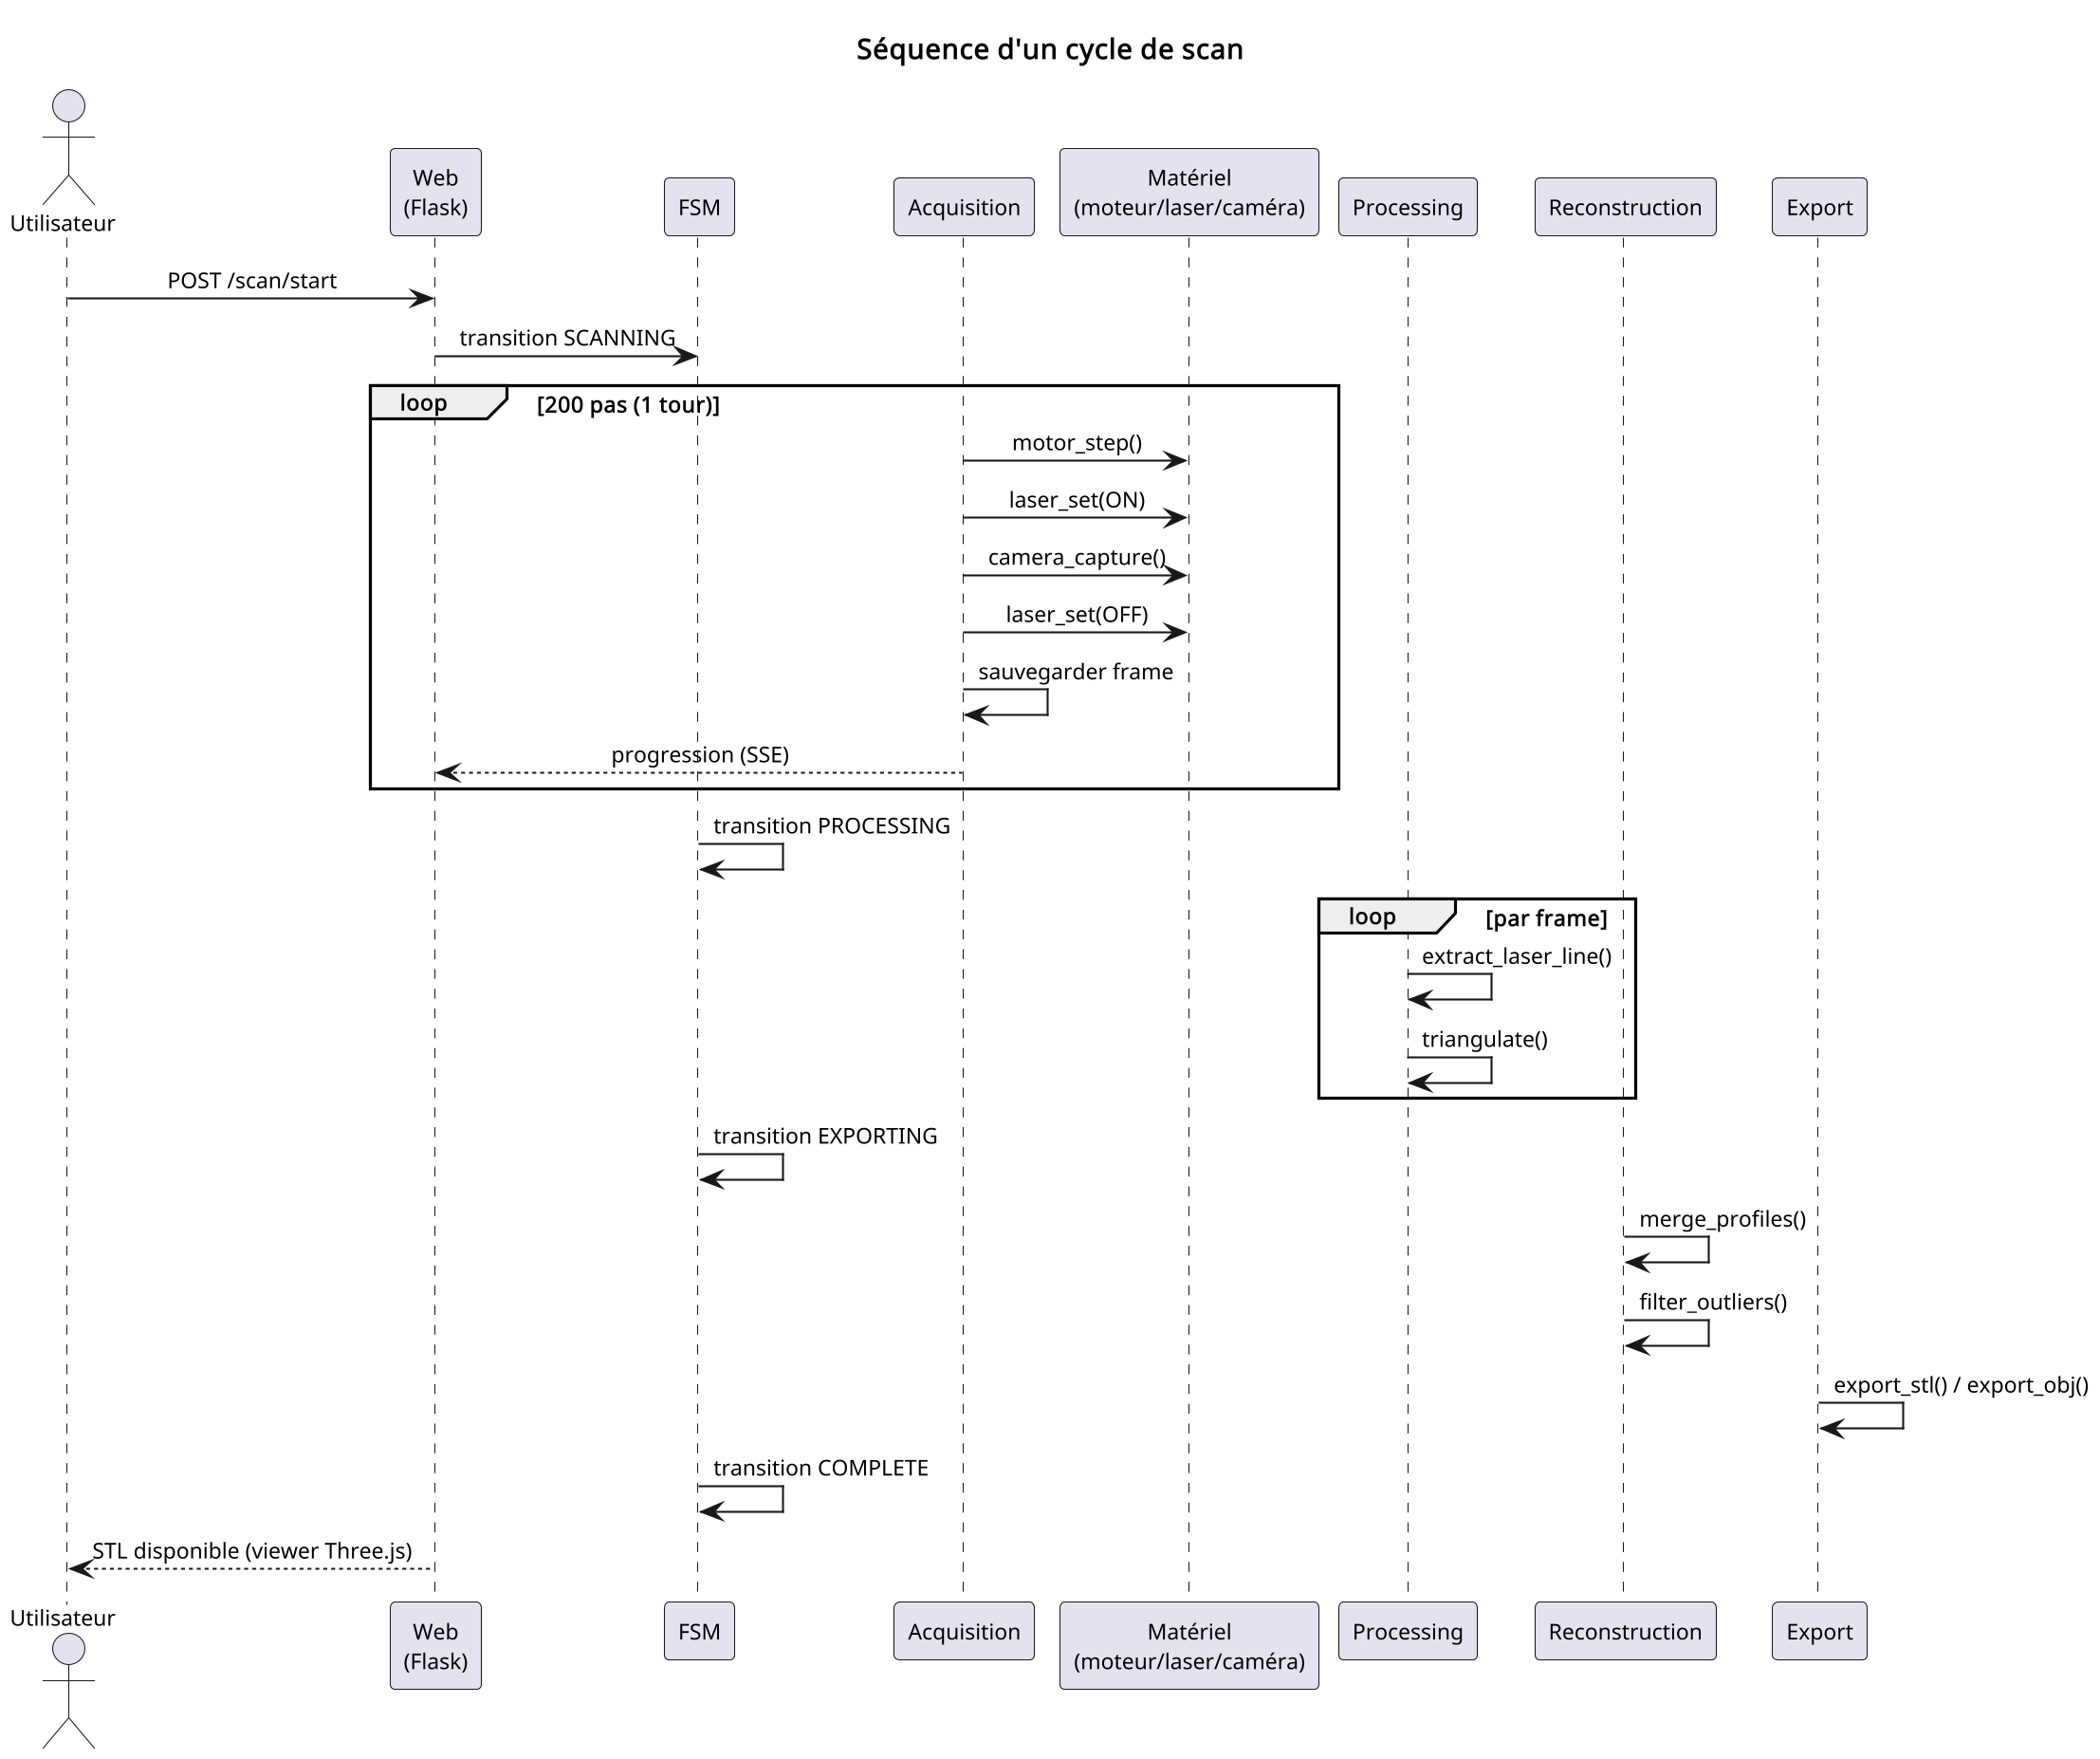
\includegraphics[width=\linewidth,height=6.05cm,keepaspectratio]{sequence_scan.png}
    \end{column}
    \begin{column}{0.24\textwidth}
      \validbox{Scan lancé depuis l'interface web.}
      \vspace{0.18cm}
      \validbox{Images capturées avec ligne laser visible.}
      \vspace{0.18cm}
      \validbox{Nuage de points et STL générés.}
    \end{column}
  \end{columns}
\end{frame}

\begin{frame}{Interface et démonstration}{Scénario prévu pendant la présentation}
  \begin{columns}[T,onlytextwidth]
    \begin{column}{0.47\textwidth}
      \placeholder{4.8cm}{Capture souhaitée : interface web pendant ou après un scan, avec progression et viewer 3D. Nom conseillé : \texttt{interface\_scan.png}.}
    \end{column}
    \begin{column}{0.49\textwidth}
      \begin{enumerate}
        \item Placer une pièce simple sur le plateau.
        \item Lancer le scan depuis l'interface web.
        \item Montrer la progression et une image capturée.
        \item Ouvrir le fichier STL généré dans le viewer.
      \end{enumerate}

      \vspace{0.3cm}
      \tagbox{softblue}{Durée visée}\quad 2 à 3 minutes\\[0.25cm]
      \tagbox{softgreen}{Message}\quad La chaîne complète fonctionne déjà sur le prototype réel.
    \end{column}
  \end{columns}
\end{frame}

\begin{frame}{Résultat 1 : forme cylindrique}{Cas favorable pour le prototype actuel}
  \begin{columns}[T,onlytextwidth]
    \begin{column}{0.31\textwidth}
      \placeholder{4.25cm}{Image caméra réelle avec ligne laser visible sur cylindre. Nom : \texttt{cylindre\_image\_laser.jpg}.}
    \end{column}
    \begin{column}{0.31\textwidth}
      \placeholder{4.25cm}{Vue du nuage de points ou points extraits du cylindre. Nom : \texttt{cylindre\_nuage.png}.}
    \end{column}
    \begin{column}{0.31\textwidth}
      \placeholder{4.25cm}{Capture du STL cylindre obtenu. Nom : \texttt{cylindre\_stl.png}.}
    \end{column}
  \end{columns}

  \vspace{0.2cm}
  \validbox{Sur une forme simple et régulière, le pipeline produit un résultat exploitable et cohérent qualitativement.}
\end{frame}

\begin{frame}{Résultat 2 : pièce anguleuse}{Un cas qui révèle la limite physique}
  \begin{columns}[T,onlytextwidth]
    \begin{column}{0.48\textwidth}
      \placeholder{4.8cm}{Photo ou capture du scan d'une pièce rectangulaire/carrée montrant les zones manquantes. Nom : \texttt{rectangle\_limite.png}.}
    \end{column}
    \begin{column}{0.48\textwidth}
      \begin{itemize}
        \item Certaines orientations masquent la ligne laser à la caméra.
        \item Les points absents ne peuvent pas être récupérés par un simple réglage logiciel.
        \item Le STL devient fragile dès que le nuage contient des trous structurés.
      \end{itemize}

      \vspace{0.25cm}
      \limitbox{La configuration mono-caméra est insuffisante pour couvrir toutes les zones visibles par le laser sur des pièces anguleuses.}
    \end{column}
  \end{columns}
\end{frame}

\begin{frame}{Analyse de l'occultation}{Le laser touche la pièce, mais la caméra ne voit pas toujours le point}
  \begin{columns}[T,onlytextwidth]
    \begin{column}{0.52\textwidth}
      \begin{tikzpicture}[scale=0.98, every node/.style={font=\small}]
        \draw[fill=softblue,draw=linegray] (0,0) rectangle (6.3,4.5);
        \begin{scope}[rotate around={30:(3.25,1.7)}]
          \draw[fill=white,draw=deepblue,thick] (2.6,1.05) rectangle (3.9,2.35);
        \end{scope}
        \draw[heigred,very thick] (0.7,3.8) -- (2.84,2.59);
        \draw[deepblue,very thick,dashed] (5.7,3.8) -- (3.35,1.32);
        \draw[deepblue,very thick] (5.7,3.8) -- (4.14,2.05);
        \draw[heigred,fill=heigred] (2.84,2.59) circle (0.06);
        \node[heigred,align=center] at (1.2,4.1) {laser};
        \node[deepblue,align=center] at (5.45,4.1) {caméra};
        \node[align=center] at (3.2,0.55) {face de l'objet};
        \node[align=center,text width=2.2cm] at (4.85,1.35) {zone masquée depuis la caméra};
      \end{tikzpicture}
    \end{column}
    \begin{column}{0.44\textwidth}
      \begin{itemize}
        \item Deux familles de pertes sont séparées.
        \item \textbf{Perte physique} : ligne invisible pour la caméra.
        \item \textbf{Perte algorithmique} : ligne visible mais seuil ou extraction imparfaits.
      \end{itemize}

      \vspace{0.25cm}
      \nextbox{La suite doit traiter les deux causes séparément : vue complémentaire et amélioration de l'extraction.}
    \end{column}
  \end{columns}
\end{frame}

\begin{frame}{État des sous-systèmes}{Maturité au rapport intermédiaire}
  \small
  \begin{tabularx}{\linewidth}{@{}p{3.2cm}p{2.2cm}X@{}}
    \toprule
    \textbf{Sous-système} & \textbf{Maturité} & \textbf{État actuel} \\
    \midrule
    Mécanique & \maturity{3}{deepblue} & Prototype fabriqué ; stabilité, centrage et support deuxième caméra à améliorer. \\
    Électronique & \maturity{3}{deepblue} & Alimentation et commandes testées ; intégration complète et interlock à finaliser. \\
    Acquisition & \maturity{4}{deepblue} & Scan réel, capture et sauvegarde d'images fonctionnels. \\
    Extraction laser & \maturity{3}{deepblue} & Majorité des points visibles récupérée ; réglages à améliorer. \\
    Nuage de points & \maturity{4}{deepblue} & Rendu propre et exploitable pour l'analyse. \\
    Export STL & \maturity{2}{heigred} & Fonctionnel, mais fragile sur formes non cylindriques. \\
    Interface web & \maturity{3}{deepblue} & Démontrable, encore orientée debug. \\
    Validation métrique & \maturity{1}{heigred} & Protocole formel à réaliser avec objets étalons. \\
    \bottomrule
  \end{tabularx}
\end{frame}

\begin{frame}{Performances intermédiaires}{Ce qui est mesuré, observé ou encore à mesurer}
  \begin{columns}[T,onlytextwidth]
    \begin{column}{0.55\textwidth}
      \begin{tabularx}{\linewidth}{@{}p{3.4cm}X@{}}
        \toprule
        \textbf{Indicateur} & \textbf{État actuel} \\
        \midrule
        Temps de scan & Environ 1 à 1,5 min observé \\
        Largeur/profondeur & Cohérentes par contrôle manuel \\
        Hauteur & Déformation vers le haut à diagnostiquer \\
        Répétabilité & Non mesurée formellement \\
        Précision absolue & Non mesurée formellement \\
        Ergonomie & Interface démontrable, à simplifier \\
        \bottomrule
      \end{tabularx}
    \end{column}
    \begin{column}{0.40\textwidth}
      \validbox{La contrainte de temps inférieur à 10 minutes est atteignable avec une marge importante.}
      \vspace{0.2cm}
      \limitbox{La qualité géométrique finale reste l'axe prioritaire de la prochaine phase.}
    \end{column}
  \end{columns}
\end{frame}

\begin{frame}{Sécurité et points ouverts}{Conserver une démonstration maîtrisée}
  \begin{columns}[T,onlytextwidth]
    \begin{column}{0.61\textwidth}
      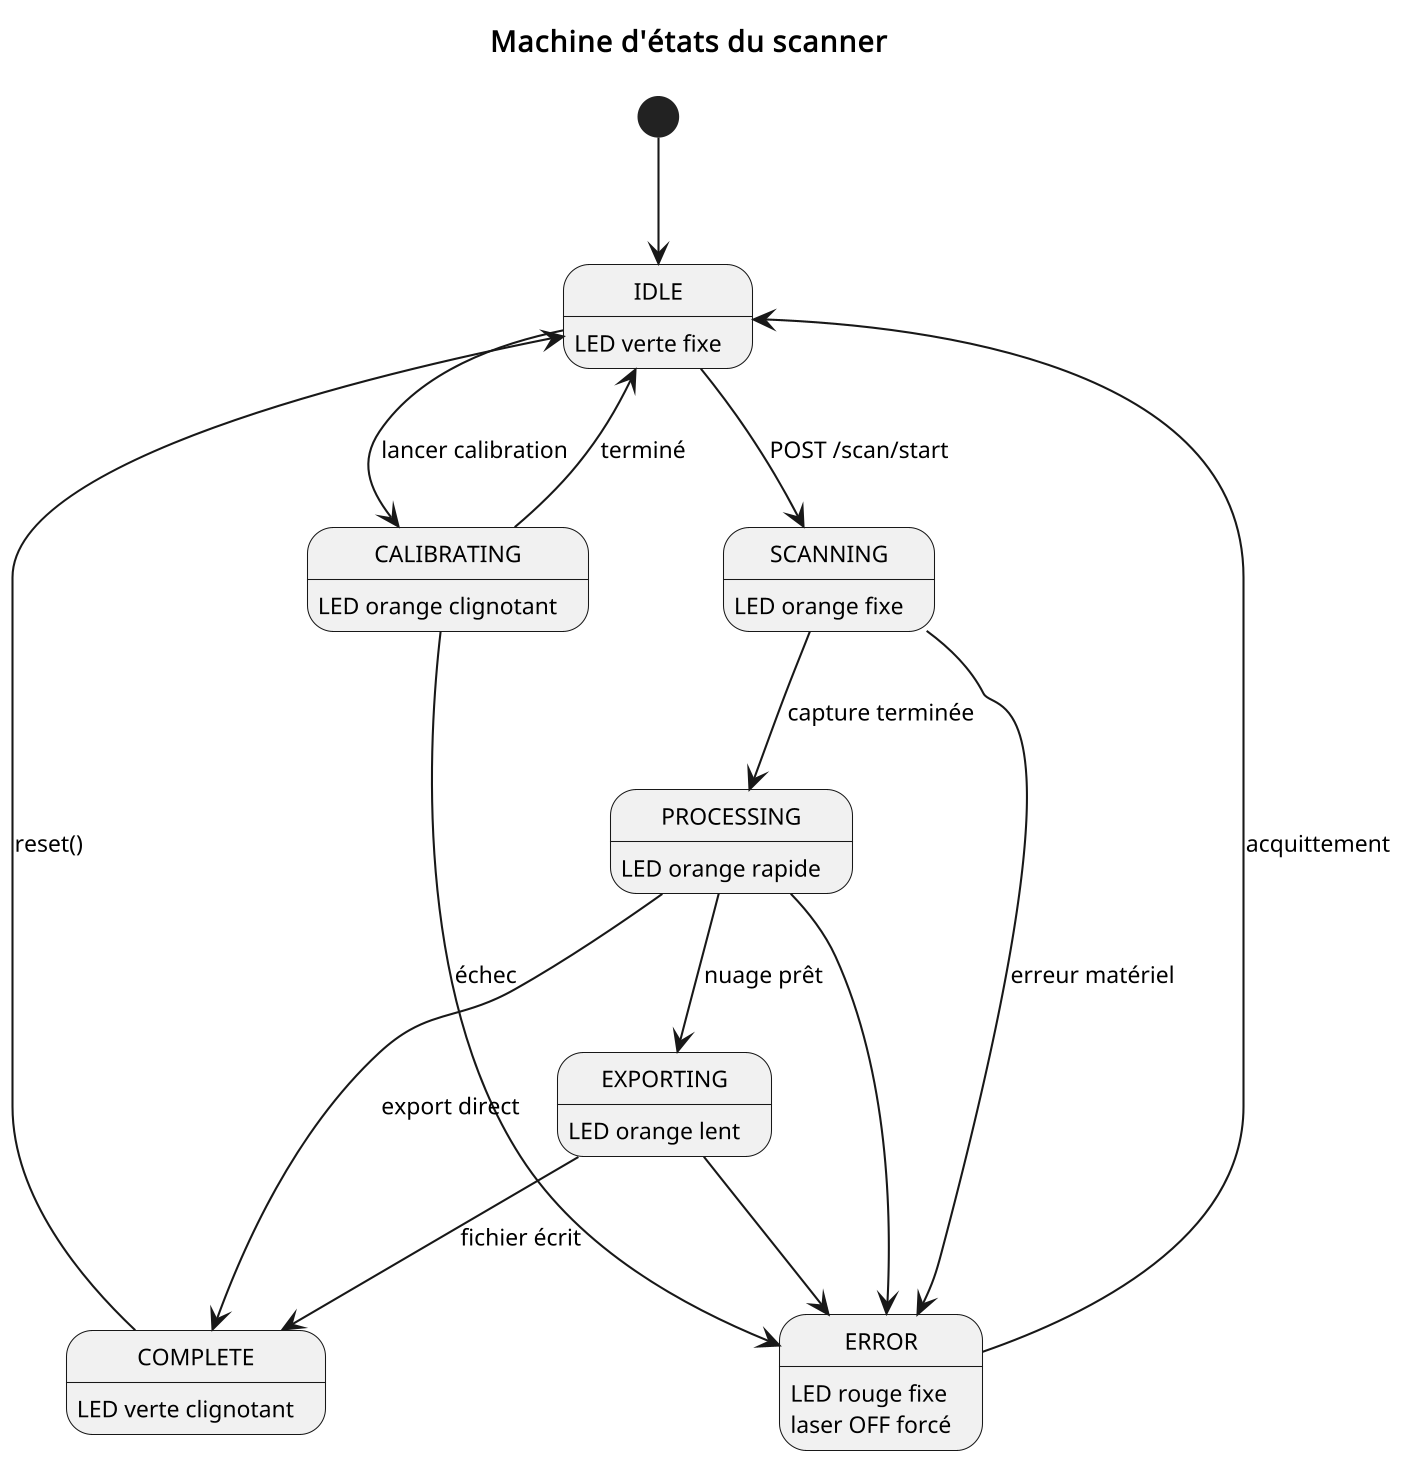
\includegraphics[width=\linewidth,height=5.85cm,keepaspectratio]{machine_etats.png}
    \end{column}
    \begin{column}{0.35\textwidth}
      \small
      \begin{itemize}
        \item Laser désactivé au démarrage.
        \item Coupure automatique en état \texttt{ERROR}.
        \item Boîte fermée pour confiner lumière et pièces mobiles.
        \item Interlock capot absent sur le prototype de test.
        \item Petites ouvertures de la boîte à isoler.
      \end{itemize}

      \vspace{0.2cm}
      \limitbox{La démonstration reste encadrée ; la version utilisateur nécessite les sécurités matérielles finales.}
    \end{column}
  \end{columns}
\end{frame}

\begin{frame}{Décision technique : deuxième caméra}{Réduire les zones invisibles}
  \begin{columns}[T,onlytextwidth]
    \begin{column}{0.50\textwidth}
      \placeholder{4.9cm}{Schéma ou photo annotée souhaitée : caméra actuelle à gauche vers le haut, caméra USB ajoutée à droite vers le bas. Nom : \texttt{schema\_deux\_cameras.png}.}
    \end{column}
    \begin{column}{0.46\textwidth}
      \begin{itemize}
        \item La caméra actuelle ne voit pas toutes les zones éclairées.
        \item Une deuxième caméra USB apporterait une vue complémentaire.
        \item Les deux nuages devront être calibrés et fusionnés dans un même repère.
        \item Les cavités profondes resteront à évaluer après ce test.
      \end{itemize}

      \vspace{0.25cm}
      \nextbox{Priorité technique : valider expérimentalement le gain avant de figer l'architecture finale.}
    \end{column}
  \end{columns}
\end{frame}

\begin{frame}{Plan de validation finale}{Passer d'une preuve qualitative à des mesures}
  \begin{columns}[T,onlytextwidth]
    \begin{column}{0.48\textwidth}
      \begin{itemize}
        \item Scanner des objets étalons imprimés et mesurés.
        \item Comparer largeur, profondeur et hauteur.
        \item Répéter plusieurs scans d'un même objet.
        \item Mesurer le temps complet pièce posée $\rightarrow$ fichier exporté.
      \end{itemize}
    \end{column}
    \begin{column}{0.48\textwidth}
      \begin{tabularx}{\linewidth}{@{}p{3.2cm}X@{}}
        \toprule
        \textbf{Critère} & \textbf{Cible} \\
        \midrule
        Temps & $<10$ min \\
        Précision & Erreur moyenne $\leq 2$ mm \\
        Répétabilité & Écart-type $\leq 1$ mm \\
        Utilisation & Prise en main $<10$ min \\
        Export & STL ou OBJ exploitable \\
        \bottomrule
      \end{tabularx}
    \end{column}
  \end{columns}
\end{frame}

\begin{frame}{Roadmap jusqu'au rendu final}{Itérations ciblées}
  \begin{tikzpicture}[x=1cm,y=1cm,every node/.style={font=\small}]
    \draw[very thick,deepblue] (0,0) -- (13.6,0);
    \foreach \x/\title/\desc in {
      0.5/{1. Deuxième caméra}/{Test mécanique et acquisition USB},
      3.1/{2. Calibration}/{Fusion dans un repère commun},
      5.7/{3. Extraction}/{Séparer seuils et occultations},
      8.3/{4. Maillage}/{Tester reconstruction robuste},
      10.9/{5. Validation}/{Objets étalons et mesures},
      13.1/{6. Finition}/{Sécurité, interface, rapport final}
    } {
      \fill[heigred] (\x,0) circle (0.08);
      \node[align=center,text width=2.15cm,anchor=north] at (\x,-0.22) {\textbf{\title}\\\scriptsize\textcolor{mutedgray}{\desc}};
    }
  \end{tikzpicture}

  \vspace{1.9cm}
  \nextbox{L'objectif n'est plus de prouver que le cycle existe : il faut maintenant fiabiliser la géométrie, mesurer et sécuriser l'usage.}
\end{frame}

\begin{frame}{Conclusion}{Acquis, limites, prochaine étape}
  \begin{columns}[T,onlytextwidth]
    \begin{column}{0.32\textwidth}
      \validbox{Prototype réel assemblé, scan complet lancé depuis l'interface web, export STL obtenu.}
    \end{column}
    \begin{column}{0.32\textwidth}
      \limitbox{Les formes anguleuses exposent une limite de visibilité et un maillage STL encore fragile.}
    \end{column}
    \begin{column}{0.32\textwidth}
      \nextbox{Tester une deuxième caméra, améliorer l'extraction, remplacer le maillage fragile et valider par mesures.}
    \end{column}
  \end{columns}

  \vspace{0.55cm}
  \begin{center}
    \Large\textbf{\textcolor{deepblue}{Message intermédiaire}}\\[0.15cm]
    \normalsize Le projet est démontrable, les limites principales sont identifiées, et la suite est structurée autour de risques techniques concrets.
  \end{center}
\end{frame}

\end{document}
